%! Author = Len Washington III
%! Date = 10/31/2023

% Preamble
\documentclass[chapter=7,section=5]{math252homework}

% Document
\begin{document}

\customsection{7.5}{sec:7.5}

In Problems 1--12 use the Laplace transform to solve the given initial-value problem.
\begin{problems}[start=3]
	\problem \[ y'' + y = \delta(t-2\pi),\ivpsep y(0)=0,\ivpsep y'(0)=1 \]
	% TODO: Problem 3
	\setcounter{problemsi}{7}
	\problem \[ y'' - 2y' = 1 + \delta(t-2),\ivpsep y(0)=0,\ivpsep y'(0)=1 \]
	% TODO: Problem 8
	\problem \[ y'' + 4y' + 5y = \delta(t-2\pi),\ivpsep y(0)=0,\ivpsep y'(0)=0 \]
	% TODO: Problem 9
	\setcounter{problemsi}{10}
	\problem \[ y'' + 4y' + 13y = \delta(t-\pi) + \delta(t - 3\pi),\ivpsep y(0)=1,\ivpsep y'(0)=0 \]
	\answer{\begin{equation*}
	\begin{aligned}
		y'' + 4y' + 13y &= \delta(t-\pi) + \delta(t - 3\pi)\\
		\laplace[y''] + 4\laplace[y'] + 13\laplace[y] &= \laplace[\delta(t-\pi)] + \laplace[\delta(t - 3\pi)]\\
		s^{2}\laplace[y] - sy(0) - y'(0) + 4\left( s\laplace[y] - y(0) \right) + 13\laplace[y] &= e^{-\pi s} + e^{-3\pi s}\\
		s^{2}\laplace[y] - s(1) - 0 + 4s\laplace[y] - 4 + 13\laplace[y] &= e^{-\pi s} + e^{-3\pi s}\\
		s^{2}\laplace[y] + 4s\laplace[y] + 13\laplace[y] &= e^{-\pi s} + e^{-3\pi s} + s + 4\\
		\laplace[y]\left( s^{2} + 4s + 13 \right) &= e^{-\pi s} + e^{-3\pi s} + s + 4\\
	\end{aligned}
	\end{equation*}\begin{equation*}
	\begin{aligned}
		\laplace[y] &= \frac{e^{-\pi s} + e^{-3\pi s} + s + 4}{s^{2} + 4s + 13}\\
					&= \frac{e^{-\pi s} + e^{-3\pi s} + s + 4}{s^{2} + 4s + 4 + 9}\\
					&= \frac{e^{-\pi s} + e^{-3\pi s} + s + 4}{(s+2)^{2} + 9}\\
					&= \frac{e^{-\pi s}}{(s+2)^{2} + 9} + \frac{e^{-3\pi s}}{(s+2)^{2} + 9} + \frac{s + 4}{(s+2)^{2} + 9}\\
	\end{aligned}
	\end{equation*}\begin{equation*}
	\begin{aligned}
		y &= \laplacei[\frac{e^{-\pi s}}{(s+2)^{2} + 9}] + \laplacei[\frac{e^{-3\pi s}}{(s+2)^{2} + 9}] + \laplacei[\frac{s + 4}{(s+2)^{2} + 9}]\\
		  &= \laplacei[\frac{e^{-\pi s}}{(s+2)^{2} + 9}] + \laplacei[\frac{e^{-3\pi s}}{(s+2)^{2} + 9}]
		   \\&+ \laplacei[\frac{s + 2}{(s+2)^{2} + 9}] + \laplacei[\frac{2}{(s+2)^{2} + 9}]\\
		  &= \laplacei[\frac{e^{-\pi s}}{(s+2)^{2} + 9}] + \laplacei[\frac{e^{-3\pi s}}{(s+2)^{2} + 9}]
		   \\&+ \laplacei[\frac{s}{s + 3^{2}}\bigg|_{s\rightarrow s+2}] + \frac{2}{3}\laplacei[\frac{3}{s^{2} + 3^{2}}]\bigg|_{s\rightarrow s+2}\\
		  &= \laplacei[\frac{e^{-\pi s}}{(s+2)^{2} + 9}] + \laplacei[\frac{e^{-3\pi s}}{(s+2)^{2} + 9}] + e^{-2t}\cos(3t) + \frac{2}{3}e^{-2t}\sin(3t)\\
	\end{aligned}
	\end{equation*}}
	% TODO: Problem 11
\end{problems}

\customsection{3.3}{sec:3.3}
\setcounter{chapter}{3}
\setcounter{section}{3}

\customsubsection{Radioactive Series}
\begin{problems}
	\problem We have not discussed methods by which systems of first-order differential equations can be solved.
	Nevertheless, systems such as (2) can be solved with no knowledge other than how to solve a single linear first-order equation.
	Find a solution of (2) subject to the initial conditions $x(0)=x_{0}$, $y(0)=0$, $z(0)=0$.
	% TODO: Problem 1
	\setcounter{problemsi}{3}
	\problem Construct a mathematical model for a radioactive series of four elements $W$, $X$, $Y$, and $Z$, where $Z$ is a stable element.
	% TODO: Problem 4
\end{problems}

\customsubsection{Mixtures}
\begin{problems}[start=7]
	\problem Consider two tanks $A$ and $B$, with liquid being pumped in and out at the same rates, as described by the system of equations (3).
	What is the system of differential equations if, instead of pure water, a brine solution containing 2 pounds of salt per gallon is pumped into tank $A$?
	% TODO: Problem 7
	\problem Use the information given in \hyperref[fig:3.3.8]{Figure~3.3.8} to construct a mathematical model for the number of pounds of salt $x_{1}(t)$, $x_{2}(t)$, and $x_{3}(t)$ at time $t$ in tanks $A$, $B$, and $C$, respectively.
	\begin{figure}[H]
		\centering
		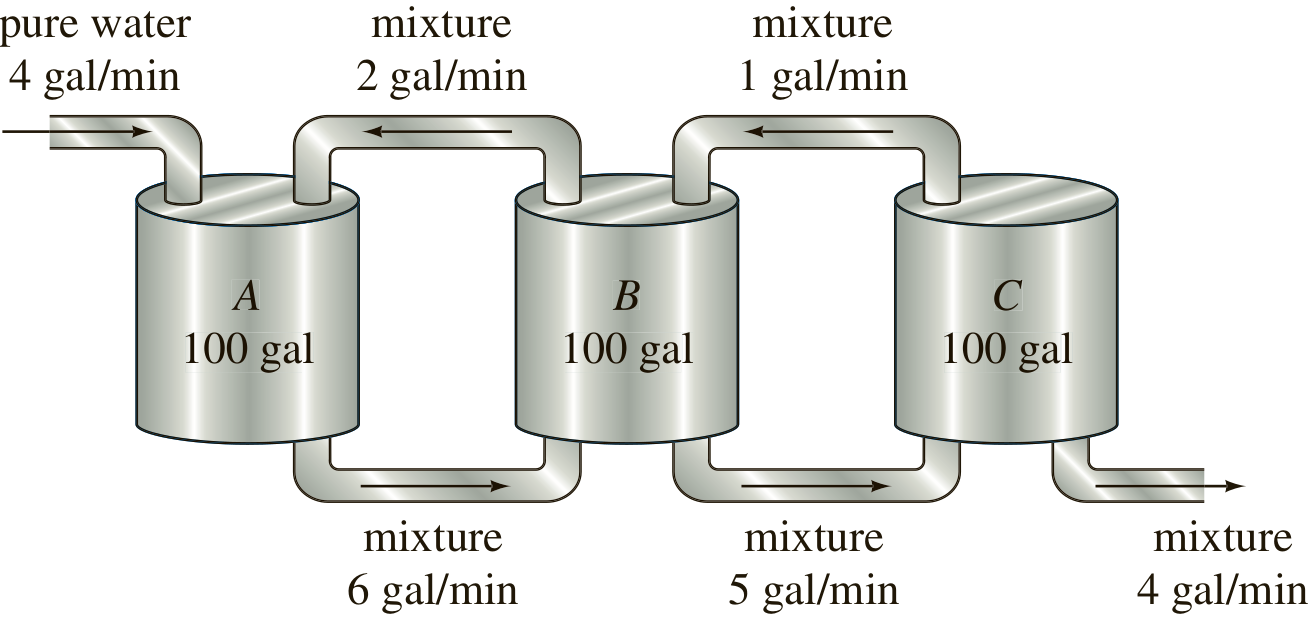
\includegraphics[width=\textwidth]{3.3.8}
		\caption{Mixing tanks in Problem~\hyperref[prb:\arabic{problemsi}]{\arabic{problemsi}}.}
		\label{fig:3.3.8}
	\end{figure}
	% TODO: Problem 8
\end{problems}

\end{document}